\documentclass{standalone}
\usepackage{tikz}
\usetikzlibrary{angles,quotes,math}

\begin{document}
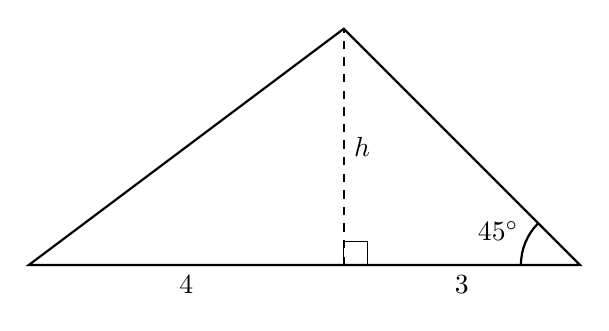
\begin{tikzpicture}
  \coordinate (a) at (0,0);
  \coordinate (b) at (4,0);
  \coordinate (c) at (7,0);
  \coordinate (d) at (4,3);
  % triangle
  \draw[thick]
  (a) -- node[below] {4}
  (b) -- node[below] {3}
  (c) pic["\(45^{\circ}\)", draw=black, -, angle eccentricity=1.5,
  angle radius=0.75cm] {angle=d--c--a} --
  (d) -- cycle;
  % height
  \draw[thick,dashed] (4,0) -- node[midway, right] {\(h\)} (4,3);
  % right angle
  \draw (4,0) rectangle ++(0.3,0.3);
\end{tikzpicture}
\end{document}
